\section{Exercício e Simulação}
\begin{frame}
\frametitle{Exercício e Simulação}
\begin{figure}[h!]
\begin{center}
    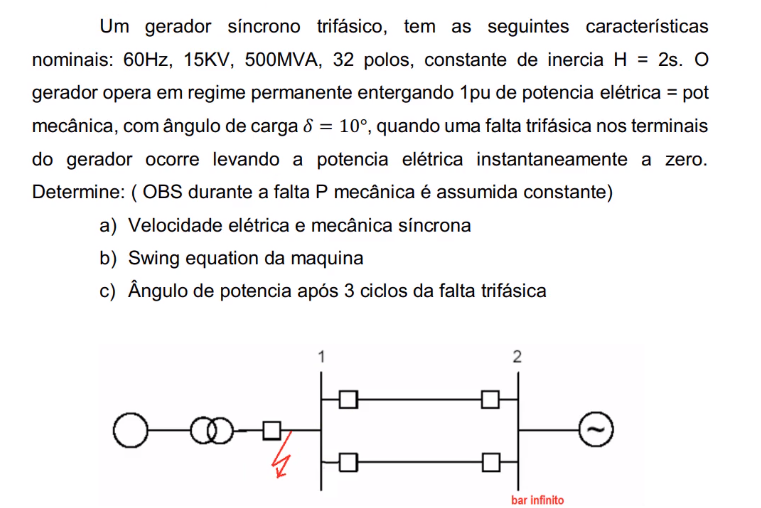
\includegraphics[width=15.3cm]{imagens/exm.png}  
\end{center}
%\caption{Resultado prático da planta em malha aberta.}
\label{maq10} 
\end{figure}
\end{frame}

\begin{frame}
\frametitle{Exercício e Simulação}
\begin{figure}[h!]
\begin{center}
    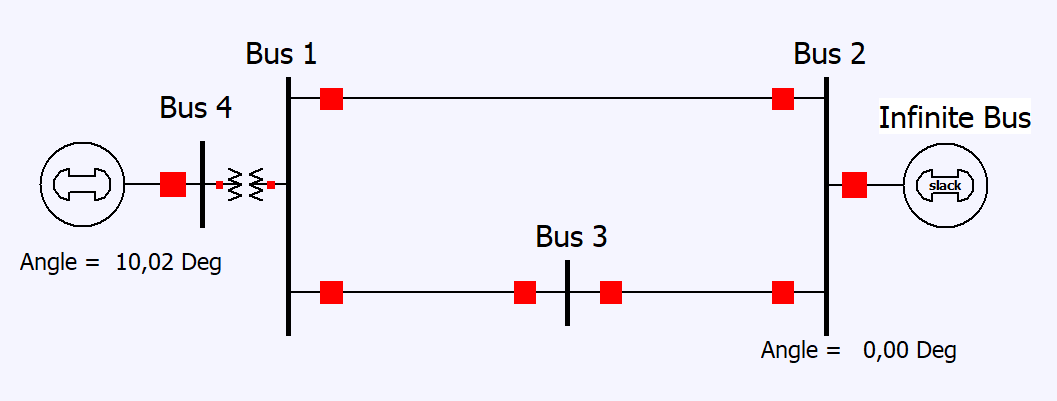
\includegraphics[width=10cm]{imagens/exm2.png}  
\end{center}
%\caption{Resultado prático da planta em malha aberta.}
\label{maq10} 
\end{figure}
\end{frame}


\begin{frame}{Resolução}
\begin{textblock*}{10pt}(20pt,60pt)

 \textbf{a)}\\
\end{textblock*}

\begin{textblock*}{10pt}(30pt,70pt)    
\small   

\begin{equation*}
 Para \hspace{2pt}f=60 \hspace{2pt}Hz
\end{equation*}
\begin{equation*}
  \omega_{ele} = 2\pi60 = \boxed{377 rad/s}
\end{equation*}

\begin{equation*}
  \omega_{mec} = \left(\frac{2}{#P} \right)\omega_{ele} = \left(\frac{2}{32} \right)377
\end{equation*}
\begin{equation*}
 \omega_{mec} = \boxed{23,56 rad/s}
\end{equation*}
 

\end{textblock*}




\begin{textblock*}{10pt}(240pt,60pt)

 \textbf{b)}\\
\end{textblock*}

\begin{textblock*}{10pt}(250pt,70pt)    
\small   

\begin{equation*}
  \frac{2H}{\omega_{sinc}}(t) \frac{d^{2} \delta(t)}{d t^2} = P_m(t)-P_e(t) -D\omega_{sinc} \frac{d \delta(t)}{d t}
\end{equation*}
\vspace{0.5pt}  
\begin{equation*}
  \boxed{\left(\frac{4}{377}\right) \frac{d^{2} \delta(t)}{d t^2} = P_m(t)-P_e(t)}
\end{equation*}
\vspace{0.5pt}
\end{textblock*}

\end{frame}

\begin{frame}{Resolução}
\begin{textblock*}{10pt}(20pt,60pt)

 \textbf{c)}\\
\end{textblock*}


\begin{textblock*}{10pt}(30pt,70pt)    
\small   


\begin{equation*}
  Para\hspace{2pt} um \hspace{2pt} t \hspace{2pt} antes \hspace{2pt} da \hspace{2pt} falta \hspace{2pt} (t^-):
\end{equation*}
\begin{textblock*}{10pt}(50pt,90pt)
\begin{equation*}
  \delta(t^-) = 10º = 0,1745 rad
\end{equation*}
\end{textblock*}
\begin{equation*}
  Para\hspace{2pt} \hspace{2pt} t \hspace{2pt} imediatamente \hspace{2pt} após \hspace{2pt} a \hspace{2pt} falta \hspace{2pt} (t):
\end{equation*}
\begin{textblock*}{10pt}(50pt,135pt)
\begin{equation*}
  \left(\frac{4}{377}\right) \frac{d^{2} \delta(t)}{d t^2} = 1-0 = 1
\end{equation*}
\begin{equation*}
   \frac{d \delta(t)}{d t} = \left(\frac{377}{4} \right)t + 0
\end{equation*}
\begin{equation*}
   \delta(t) = \left(\frac{377}{8} \right)t^2 + 0,1745
\end{equation*}
\end{textblock*}


\begin{textblock*}{10pt}(220pt,70pt)
\begin{equation*}
   t= 3 \hspace{2pt}ciclos = \frac{3 \hspace{2pt} ciclos}{60 \hspace{2pt} ciclos/s} = 0,05 \hspace{2pt}s 
\end{equation*}
\begin{equation*}
   \delta(0,05) = \left(\frac{377}{8} \right)(0,05)^2 + 0,1745
\end{equation*}
\begin{equation*}
   \delta(0,05) = 0,2923 \hspace{2pt} rad = \boxed{16,75º}
\end{equation*}


\end{textblock*}

\end{textblock*}
\end{frame}